\documentclass[a4paper, 9pt, conference]{article}

%usepackage{txfonts} % ss
%let\temp\rmdefault
%usepackage{fourier} % math & rm
%let\rmdefault\temp

%packages
\usepackage[english,spanish]{babel}
\usepackage[latin1]{inputenc}

\usepackage{amssymb}
\usepackage{amsmath}
\usepackage{mathtools}
\usepackage{zed-csp}

\usepackage[pdftex]{graphicx}

\usepackage{ragged2e}

\usepackage{hyperref}

\usepackage{framed}
\usepackage{wrapfig}
\usepackage{fancyhdr}
%\pagestyle{fancy}
%\lhead{Promoci\'on de la Econom\'ia Circular mediante un sistema de criptodivisa con incentivos}

\usepackage[table,xcdraw]{xcolor}
\usepackage{float}
\usepackage{enumitem, tasks}


\newcolumntype{a}{>{\hsize=.2\hsize\raggedleft\arraybackslash}X}
\newcolumntype{b}{>{\raggedleft\arraybackslash}X}
\newcolumntype{L}{>{\centering\arraybackslash}m{\textwidth}}


\renewcommand\thesection{\arabic{section}}
\renewcommand\thesubsection{\thesection.\arabic{subsection}}
\renewcommand\theequation{\alph{equation}}

\newtheorem{theorem}{Teorema}[section]
\newtheorem{heuristic}[theorem]{Heur\'istica}

\hypersetup{
	%frenchlinks=true,
	linktocpage=true,
	colorlinks=false,
	%linkcolor=tec,%=red,%black!40,
	%citecolor=tec,%=red,
	%filecolor=tec,%black,
	%urlcolor=tec,%black,
	%linkbordercolor={.89 .13 .21},
	%citebordercolor={.41 .85 .15},
	%urlbordercolor={0 0 1},
	pdftitle={Informe final} %,
	%pdfpagemode=FullScreen
}

\graphicspath{{img/}}
%\setlength{\parskip}{2mm}

\begin{document}

\title{Producci\'on y an\'alisis de datos referentes al presupuesto del Ministerio de Educaci\'on P\'ublica de Costa Rica por oferta educativa, Informe final.}

\author{
	Wilberth Castro \\
	\small{\texttt{wilz04@gmail.com}}
}

\date{\small{19 de marzo 2024}}

\maketitle


\begin{abstract}
	Este documento contiene el informe final sobre el proceso de producci\'on y an\'alisis de datos referentes al presupuesto del Ministerio de Educaci\'on P\'ublica de Costa Rica por oferta educativa. Este informe final incluye (1) el an\'alisis de los datos referentes al presupuesto del ministerio por oferta educativa, (2) los resultados de los principales indicadores del an\'alisis presupuestal, (3) un informe sobre las tendencias y sugerencias clave para la toma de decisiones y orientaci\'on del proyecto de presupuesto por programas, (4) una s\'intesis de buenas pr\'acticas, lecciones aprendidas y recomendaciones para la adecuada alimentaci\'on y procesamiento de los datos, y (5) un anexo sobre los datos desagregados que soportan el an\'alisis realizado.%(2.1) la interpretaci\'on de los resultados de los principales indicadores del an\'alisis presupuestal, 
\end{abstract}

% --------------------------------------------------------------------------------------------------------------------------------
\section{Introducci\'on} \label{sec:intro}

Este documento contiene el informe final sobre el proceso de producci\'on y an\'alisis de datos referentes al presupuesto del Ministerio de Educaci\'on P\'ublica de Costa Rica por oferta educativa. En este documento, el t\'ermino ``Ministerio'' es usado como abreviatura del t\'itulo ``Ministerio de Educaci\'on P\'ublica de Costa Rica'', y el t\'ermino ``Viceministro'' es usado como abreviatura del t\'itulo ``Viceministro de Planificaci\'on Institucional y Coordinaci\'on Regional del Ministerio de Educaci\'on P\'ublica de Costa Rica''.

En general, la planificaci\'on de un presupuesto por resultados requiere del establecimiento y la evaluaci\'on peri\'odica de indicadores de resultados, el proceso de planificaci\'on del presupuesto por resultados es un proceso iterativo que requiere revisi\'on y ajuste continuo a lo largo del tiempo, por lo tanto es fundamental disponer de datos precisos y actualizados. El tablero de indicadores permitir\'a facilitar el desarrollo de esta actividad.

% --------------------------------------------------------------------------------------------------------------------------------
\section{An\'alisis de los datos referentes al presupuesto del ministerio por oferta educativa} \label{sec:dashboard}

El ap\'endice \ref{att:dashboard} contiene una captura del componente de visualizaci\'on de indicadores, tal como ser\'an desplegados en el sitio del ministerio.%, y el ap\'endice \ref{att:database} contiene los conjuntos de datos desagregados que soportan el an\'alisis realizado.

% --------------------------------------------------------------------------------------------------------------------------------
\section{Resultados de los principales indicadores del an\'alisis presupuestal} \label{sec:settlement}

La p\'agina 6 del tablero contiene los principales indicadores del an\'alisis presupuestal. La figura \ref{fig:settlement} contiene una captura del componente de visualizaci\'on ubicado en la p\'agina 6.

\begin{figure}
	\centering
		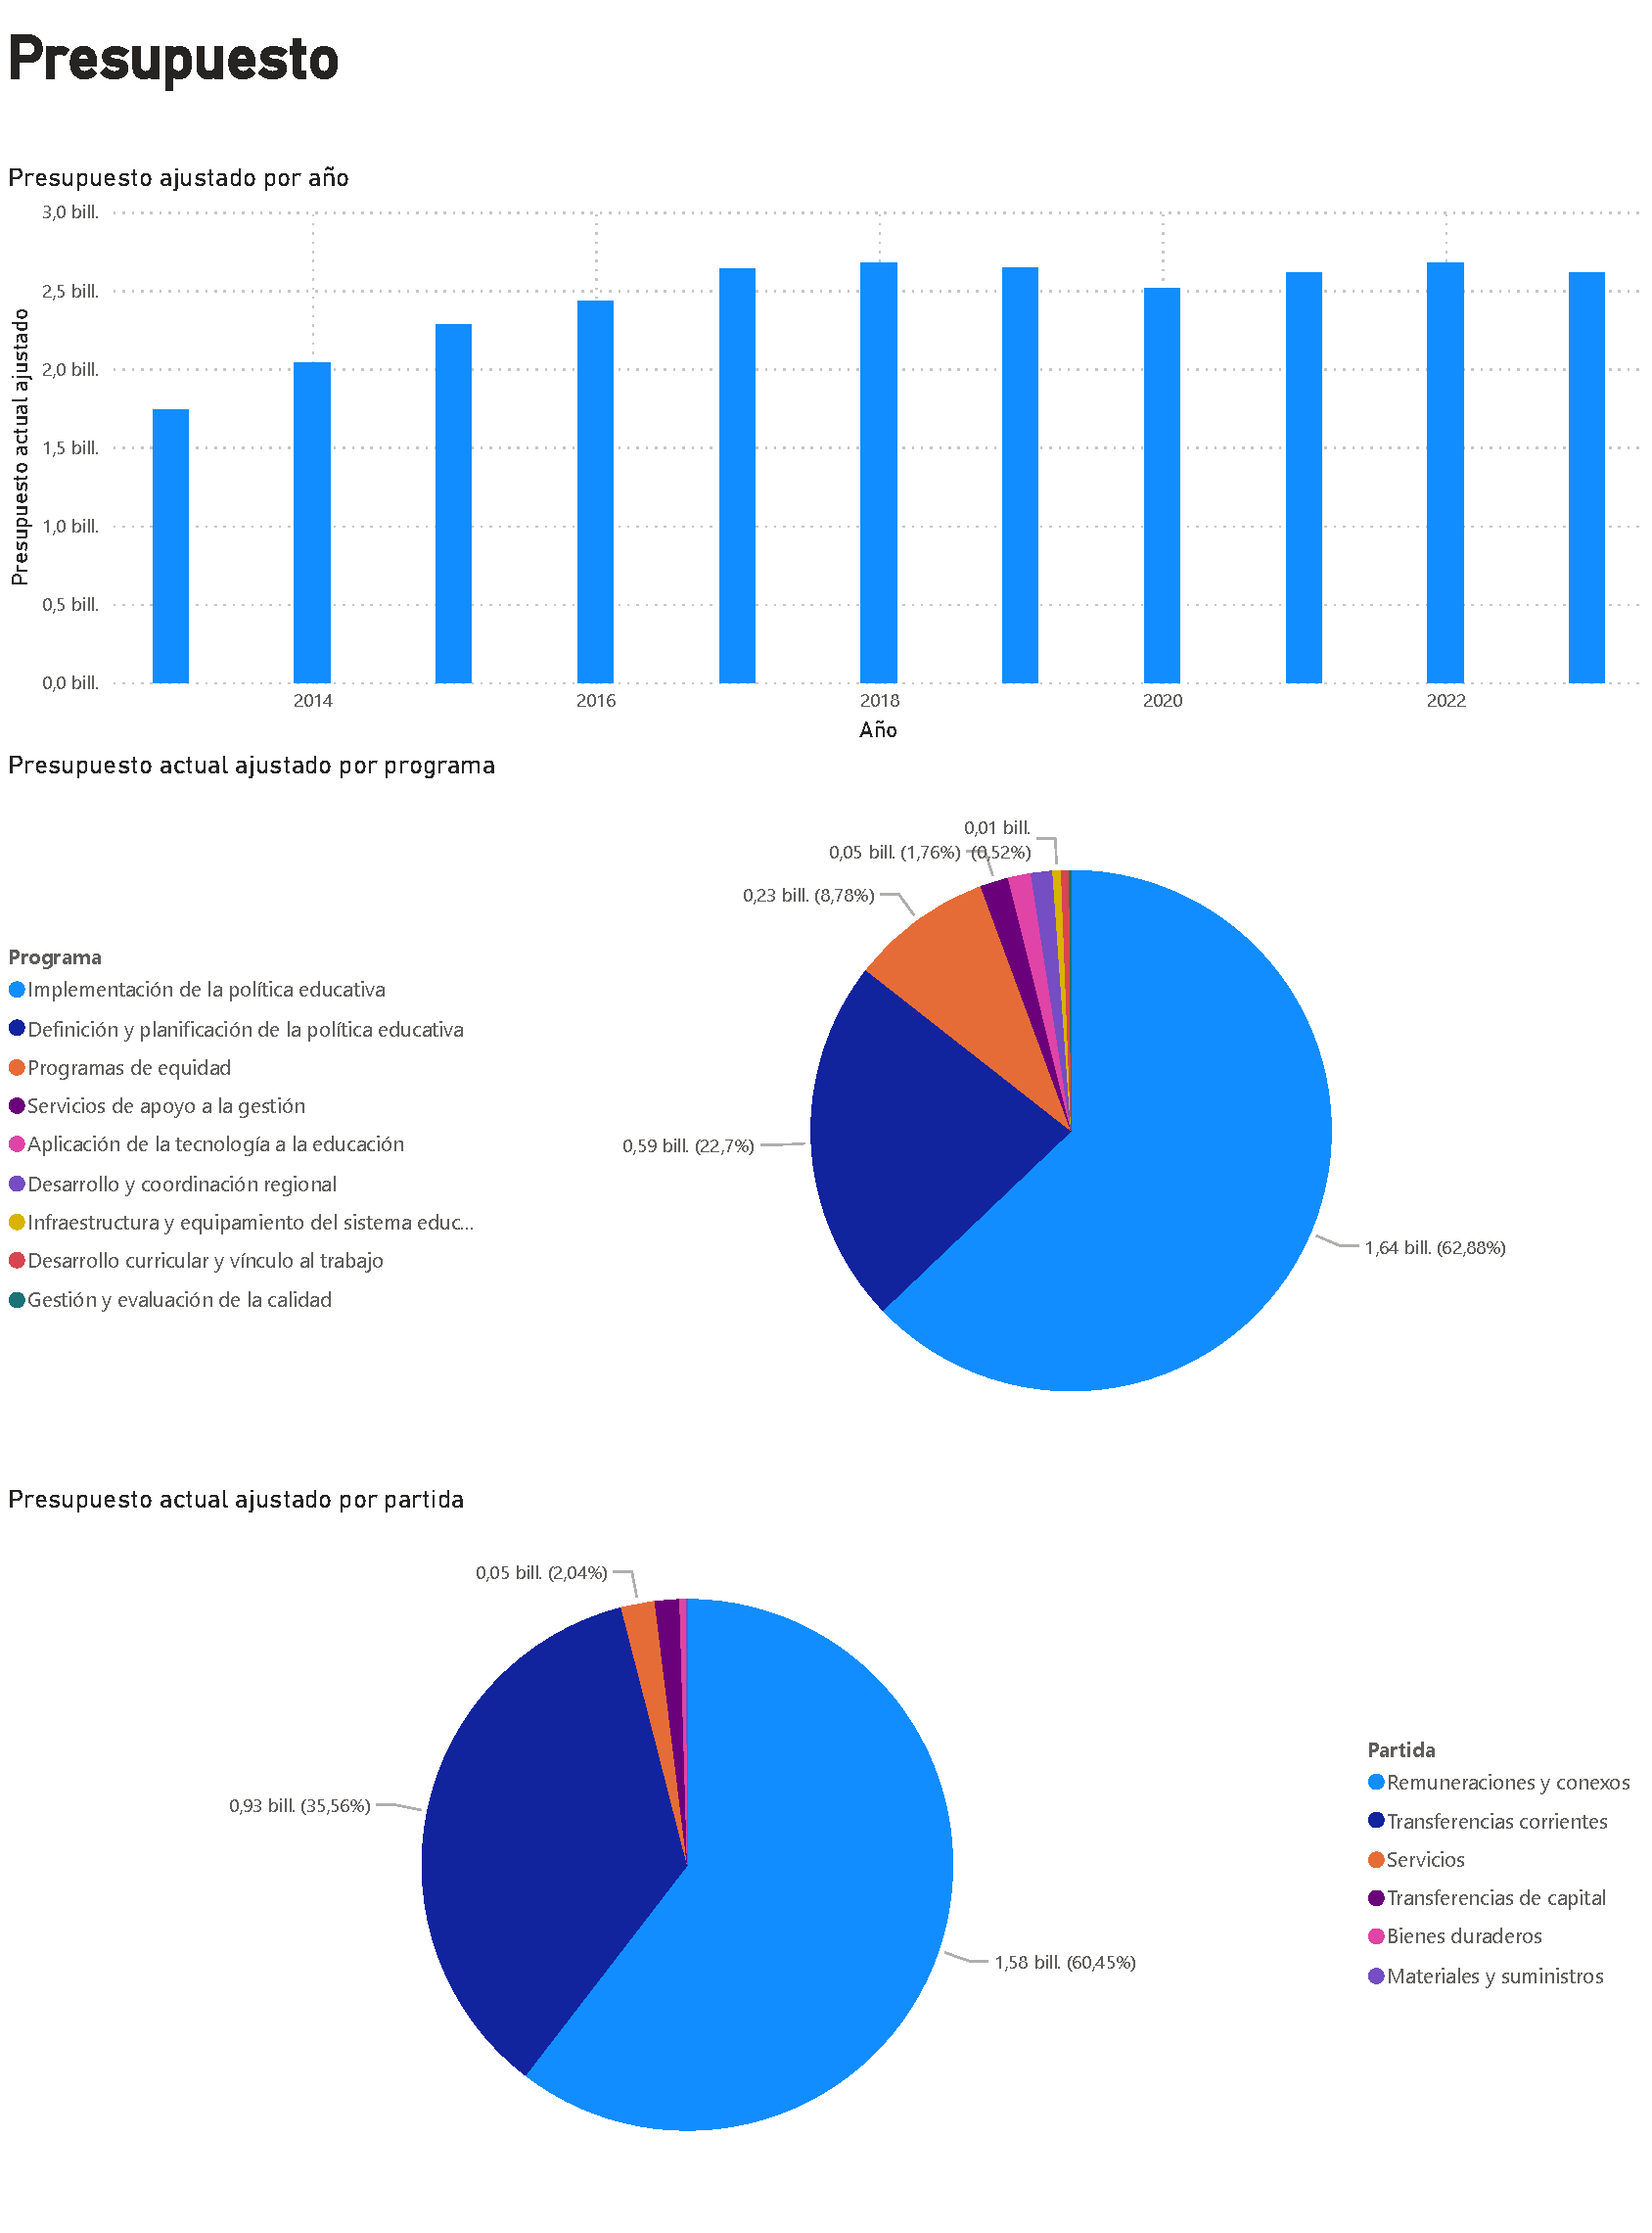
\includegraphics[width=330px, keepaspectratio=false]{settlement}
			\caption{Principales indicadores del an\'alisis presupuestal}
	\label{fig:settlement}
\end{figure}

% --------------------------------------------------------------------------------------------------------------------------------
%section{Interpretaci\'on de los resultados de los principales indicadores del an\'alisis presupuestal}

% --------------------------------------------------------------------------------------------------------------------------------
\section{Informe sobre las tendencias y sugerencias clave para la toma de decisiones y orientaci\'on del proyecto de presupuesto por programas}

En la planificaci\'on de un presupuesto por resultados, para cada objetivo estrat\'egico es necesario dise\~nar uno o varios programas que permitan satisfacer el objetivo estrat\'egico, mediante los que las actividades puedan ser realizadas y a los cuales sea posible asignar presupuesto. Sin embargo, en Costa Rica, los centros educativos reciben fondos no solo por parte del ministerio, los fondos de cada centro provienen tambi\'en de otras fuentes de ingreso, algunas establecidas por ley. El consumo de los fondos de cada centro est\'a a cargo de una junta semiaut\'onoma, y existen leyes que dificultan la reducci\'on del presupuesto, de los fondos que se transfiere cada a\~no a los centros, por lo que la implementaci\'on de un juego de programas diferente del actual mediante el que sea posible mejorar significativamente la situaci\'on actual es m\'inimamente plausible.

Una estrategia de planificaci\'on adecuada para el ministerio podr\'ia consistir en una variante de la descrita anteriormente, podr\'ia consistir en la implementaci\'on de una herramienta que permita la transmisi\'on de los objetivos estrat\'egicos a lo largo de todo el organigrama del ministerio\footnote{Actualmente hay una interrupci\'on del flujo, las juntas no tienen acceso al sistema en el que se registran los objetivos del ministerio.}, que disponga de los datos necesarios para el c\'alculo de los indicadores, que facilite el monitoreo del consumo de los fondos en tiempo real, incluyendo el consumo de los fondos de los centros educativos, y que permita registrar nuevas actividades en los programas existentes.

Cada centro educativo es administrado por una ``junta'' semiaut\'onoma. Cada junta se encarga de consumir los fondos como corresponda para el centro educativo que administra, y de reportar mensualmente al ministerio el consumo de los fondos. Actualmente, para esto se utiliza una hoja de c\'alculo, sin embargo, con frecuencia el reporte es deficiente. Claramente es necesario refinar este proceso, por lo que ser\'a necesario analizar los datos relativos al consumo de estos fondos. Ser\'a necesario cruzar la informaci\'on presupuestaria proveniente de las juntas\footnote{Es necesario establecer una relaci\'on entre cada pago efectuado y la subpartida a la que corresponde. Esta caracter\'istica podr\'ia ser implementada en el sistema de saldos del ministerio.} y la informaci\'on de las transferencias a las juntas, la \'ultima est\'a disponible en el Sistema Transferencias, Comedores y Transporte Estudiantil del ministerio, TCTE.

% --------------------------------------------------------------------------------------------------------------------------------
\section{S\'intesis de buenas pr\'acticas, lecciones aprendidas y recomendaciones para la adecuada alimentaci\'on y procesamiento de los datos}

Esta secci\'on contiene las conclusiones y recomendaciones para los objetivos espec\'ificos del proyecto.

Objetivo espec\'ifico 1: \emph{Implementar una herramienta o sistema de informaci\'on para la producci\'on y an\'alisis de datos referentes al presupuesto del MEP por nivel educativo (preescolar, primaria y secundaria)} \cite{trd}.

\begin{itemize}
	\item \textbf{Conclusiones.} Seg\'un el documento ``T\'erminos de referencia para contrataci\'on de consultor(a)/contratista individual'', el documento que contiene la fecha de entrega de cada producto \cite{trd}, el tiempo disponible para realizar las tareas de desarrollo, control de calidad y elaboraci\'on de manuales y presentaciones, es de solo dos semanas. Seg\'un la propuesta de trabajo \cite{prop}, el desarrollo de los casos de uso puede requerir de mucho m\'as tiempo, y a pesar de haber desarrollado solo los casos de uso indispensables para el desarrollo del producto 4, seg\'un el cronograma en la propuesta de trabajo \cite{prop}, el producto 3 deb\'ia ser entregado el 11 de mayo, pero fue aprobado hasta el 25 de agosto. Adem\'as del alto volumen de trabajo para el tiempo disponible, las causas del retraso fueron, como se document\'o en la secci\'on \ref{sec:binnacle}, (1) las dificultades para conseguir tiempo con quien, seg\'un el documento ``T\'erminos de referencia [...]'', debe aprobar los productos, el Viceministro \cite{trd}, y (2) la desaprobaci\'on de la matriz de Ruta de la Educaci\'on por parte del Viceministro. Finalmente, el alcance del objetivo espec\'ifico es de un 90\%, en lugar del 10\% pendiente\footnote{El 10\% pendiente corresponde a los ajustes del sistema de informaci\'on solicitados por el personal del Ministerio. La implementaci\'on de los ajustes se entregar\'a como parte del producto 4.}, se desarroll\'o un prototipo del producto 4, esto fue acordado con el Viceministro.
	\item \textbf{Recomendaciones.} En futuros proyectos, o fases de este proyecto, ser\'ia mejor realizar un an\'alisis de requerimientos antes de establecer las fechas de entrega, por otro lado, el personal del Ministerio encargado de dirigir el desarrollo y aprobar los productos debe estar suficientemente disponible para asumir estos encargos. Una fase de an\'alisis de requerimientos anterior al inicio de este proyecto hubiera podido evitar partir de una matriz de indicadores que no iba a ser aprobada.
\end{itemize}

Objetivo espec\'ifico 2: \emph{Producir insumos de an\'alisis de datos que respalden el planeamiento de un presupuesto por resultados para el Ministerio de Educaci\'on P\'ublica MEP para el a\~no 2024} \cite{trd}.

% --------------------------------------------------------------------------------------------------------------------------------
\bibliographystyle{IEEEtran}
\bibliography{refs}

% --------------------------------------------------------------------------------------------------------------------------------
\section{Ap\'endice: An\'alisis de los datos referentes al presupuesto del ministerio por oferta educativa} \label{att:dashboard}

%\begin{figure}[H]
%	\centering
%		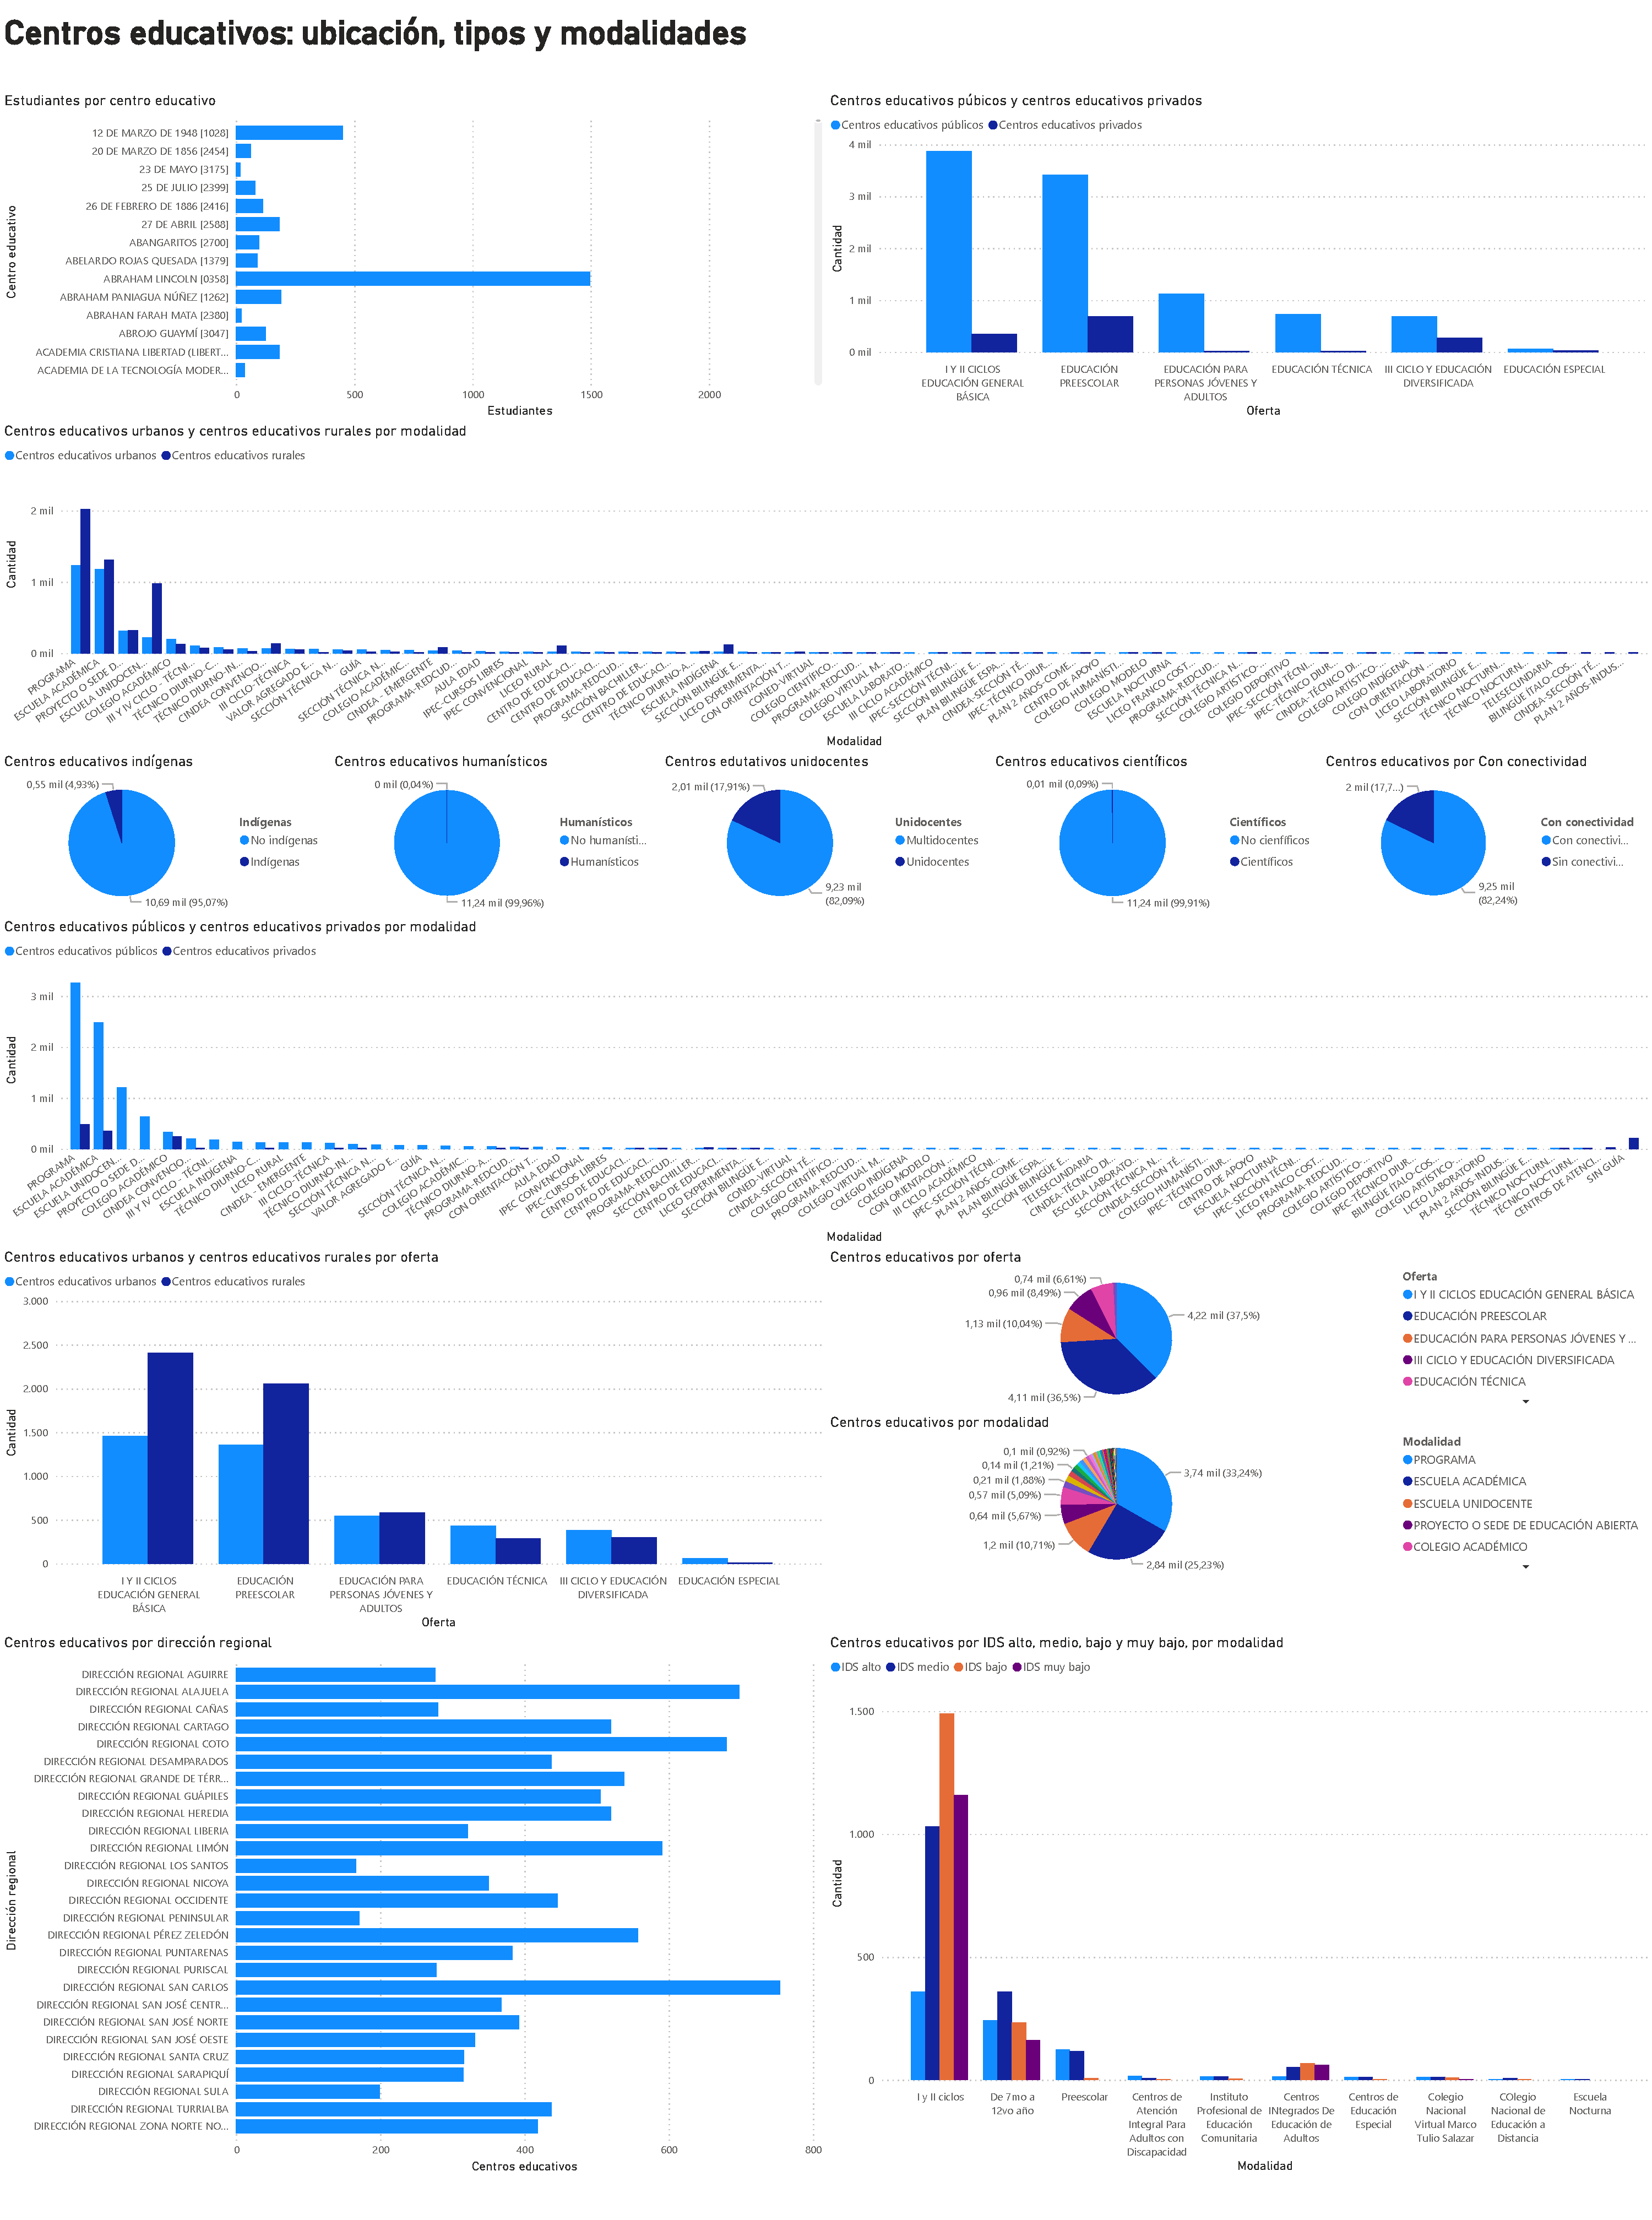
\includegraphics[width=330px, keepaspectratio=false]{landingpage}
%			\caption{Captura del componente de visualizaci\'on de indicadores}
%	\label{fig:landingpage}
%\end{figure}

% --------------------------------------------------------------------------------------------------------------------------------
%\section{Ap\'endice: Conjuntos de datos (JSON)} \label{att:database}

%\begin{table}[H]
%	\footnotesize
%	\centering
%	\caption{Provincias}
%	\label{tab:geopag_provinces}
%	\begin{tabular}{L}
%		\selectlanguage{english}
%		\justify
%		[ \{ ''C\'odigo de cat\'alogo'': ''160103'', ''C\'odigo de provincia'': ''1'', ''Provincia'': ''San Jos\'e'', ''\'Area (km2)'': ''4969.73'' \}, \{ ''C\'odigo de cat\'alogo'': ''160103'', ''C\'odigo de provincia'': ''2'', ''Provincia'': ''Alajuela'', ''\'Area (km2)'': ''9772.27'' \}, \{ ''C\'odigo de cat\'alogo'': ''160103'', ''C\'odigo de provincia'': ''3'', ''Provincia'': ''Cartago'', ''\'Area (km2)'': ''3093.23'' \}, \{ ''C\'odigo de cat\'alogo'': ''160103'', ''C\'odigo de provincia'': ''4'', ''Provincia'': ''Heredia'', ''\'Area (km2)'': ''2663.46'' \}, \{ ''C\'odigo de cat\'alogo'': ''160103'', ''C\'odigo de provincia'': ''5'', ''Provincia'': ''Guanacaste'', ''\'Area (km2)'': ''10196.32'' \}, \{ ''C\'odigo de cat\'alogo'': ''160103'', ''C\'odigo de provincia'': ''6'', ''Provincia'': ''Puntarenas'', ''\'Area (km2)'': ''11298.51'' \}, \{ ''C\'odigo de cat\'alogo'': ''160103'', ''C\'odigo de provincia'': ''7'', ''Provincia'': ''Lim\'on'', ''\'Area (km2)'': ''9176.96'' \} ]
%	\end{tabular}
%\end{table}

% --------------------------------------------------------------------------------------------------------------------------------
\end{document}
